\documentclass[12pt,a4paper]{article}
\usepackage[margin=2cm]{geometry}
\usepackage{graphicx} % Required for including pictures
\usepackage{float} % Allows putting an [H] in \begin{figure} to specify the exact location of the figure
\usepackage{wrapfig} % Allows in-line images such as the example fish picture
\usepackage{color}
\usepackage{mathtools} 
\usepackage{hyperref} % Fancy hyperrefs
\usepackage{titling} % Lets us compactify our heading
\usepackage{braket} % ???
\usepackage{cancel} % ???
\usepackage{acronym} % Acronym Package$
\usepackage{subcaption} % Captions for subfigures %
\usepackage{caption} % Caption subtlety
\usepackage[space]{grffile} % allows file names with spaces
\usepackage{lipsum} % Allows for placeholder text

\hypersetup{
colorlinks=true,
linkcolor=blue,
urlcolor=blue
}

\acrodef{stem}[STEM]{Scanning Transmission Electron Microscopy}
\acrodef{tem}[TEM]{Transmission Electron Microscope}
\acrodef{cemn}[CEMN]{Center for Electron Microscopy and Nanofabrication}
\acrodef{edx}[EDX]{Energy-dispersive X-ray spectroscopy}
\acrodef{sem}[SEM]{Scanning Electron Microscope}
\acrodef{psu}[PSU]{Portland State University}
\acrodef{hr}[HRTEM]{High Resolution \ac{tem}}
\acrodef{al}[$Al$]{Aluminum}
\acrodef{si}[$Si$]{Silicon}
\acrodef{saed}[SAED]{Select Area Electron Diffraction}
% http://staff.science.uva.nl/~polko/HOWTO/LATEX/acronym.html 

%\setlength\parindent{0pt} % Uncomment to remove all indentation from paragraphs

\graphicspath{{Data/}} % Specifies the directory where pictures are stored

\title{TEM Report 3}
\author{Bret Comnes}
\date{\today}
\posttitle{\par\end{center}}
\setlength{\droptitle}{-10pt}


\begin{document}

\maketitle

\section{Introduction} % Major section

This report will focus on the the analysis of the diffraction patterns that were acquired in the \ac{cemn} at \ac{psu} on May 23rd, 2014.  Diffraction patterns, a Kikuchi pattern and a \ac{hr} images were acquired using an FEI Technai \ac{tem}.

This paper will cover a brief conceptual/theoretical description of diffraction pattern formation.  We will then analyze diffraction patterns of a \ac{al} polycrystalline sample and a single-crystalline \ac{si} sample.  We will also analyze the lattice structure and spacing of a gold foil sample using a \ac{hr} image taken of the sample.  A Kikuchi pattern is also included and briefly discussed.

\section{Diffraction Pattern Formation} % (fold)
\label{sec:diffraction_pattern_formation}

Diffraction patterns in a \ac{tem} are formed when incoming parallel beams of electrons interact with the crystal lattice structure of a sample.  They deflect off the different planes of the structure according to brags law.  The electrons that bounce of the same plane are reflected into parallel beams.  When these parallel rays are focused through the objective lens, all the different sets of electrons traveling in parallel paths are focused into distinct bright points forming a diffraction pattern.  An example of this can be seen in Figure~\ref{fig:diff_example} which shows a simplified version of this process.  In actuality, you would want to form the image of the diffraction pattern on the actual screen or camera you are taking data with.

\begin{figure}[htbp]
  \centering
  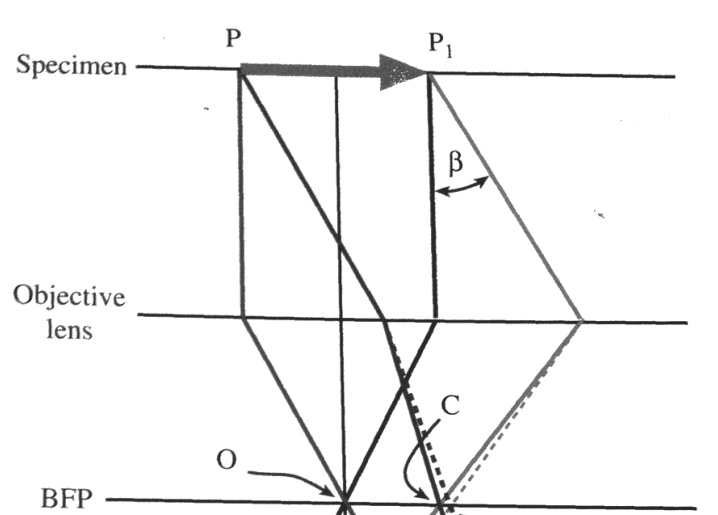
\includegraphics[width=0.5\textwidth]{data/diffpattern.PNG}
  \caption{Outgoing parallel rays focused into discrete points to form a diffraction pattern.\cite{tem}}
  \label{fig:diff_example}
\end{figure}

We can use the addition of a \ac{saed} aperture to further enhance our diffraction pattern.  The \ac{saed} aperture resides in image plane, allowing us to block out parts of our sample by literally blacking out the parts we are not interested.  Once this aperture is set in imaging mode, switching back to the diffraction pattern mode, the resulting pattern will be generated only by the parts of our sample we included in our image from the imaging plane.  This is useful when our sample is made up of a number of discrete samples and we are only interested in the diffraction pattern of a particular piece of the sample at one point.

% section diffraction_pattern_formation (end)

\subsection{Aluminum Polycrystalline Diffraction Pattern} % (fold)
\label{sub:poly}

The fist diffraction pattern we will be analyzing is from an Aluminum Polycrystalline Diffraction Pattern.  Polycrystalline samples, being made up of many crystallites, generate distinct circular diffraction pattern.  Two different images of different diffraction patterns generated from our Aluminum sample are shown in Figure~\ref{fig:aluminum}.

\begin{figure}[htbp]
  \centering
    \begin{subfigure}[b]{0.45\textwidth}
    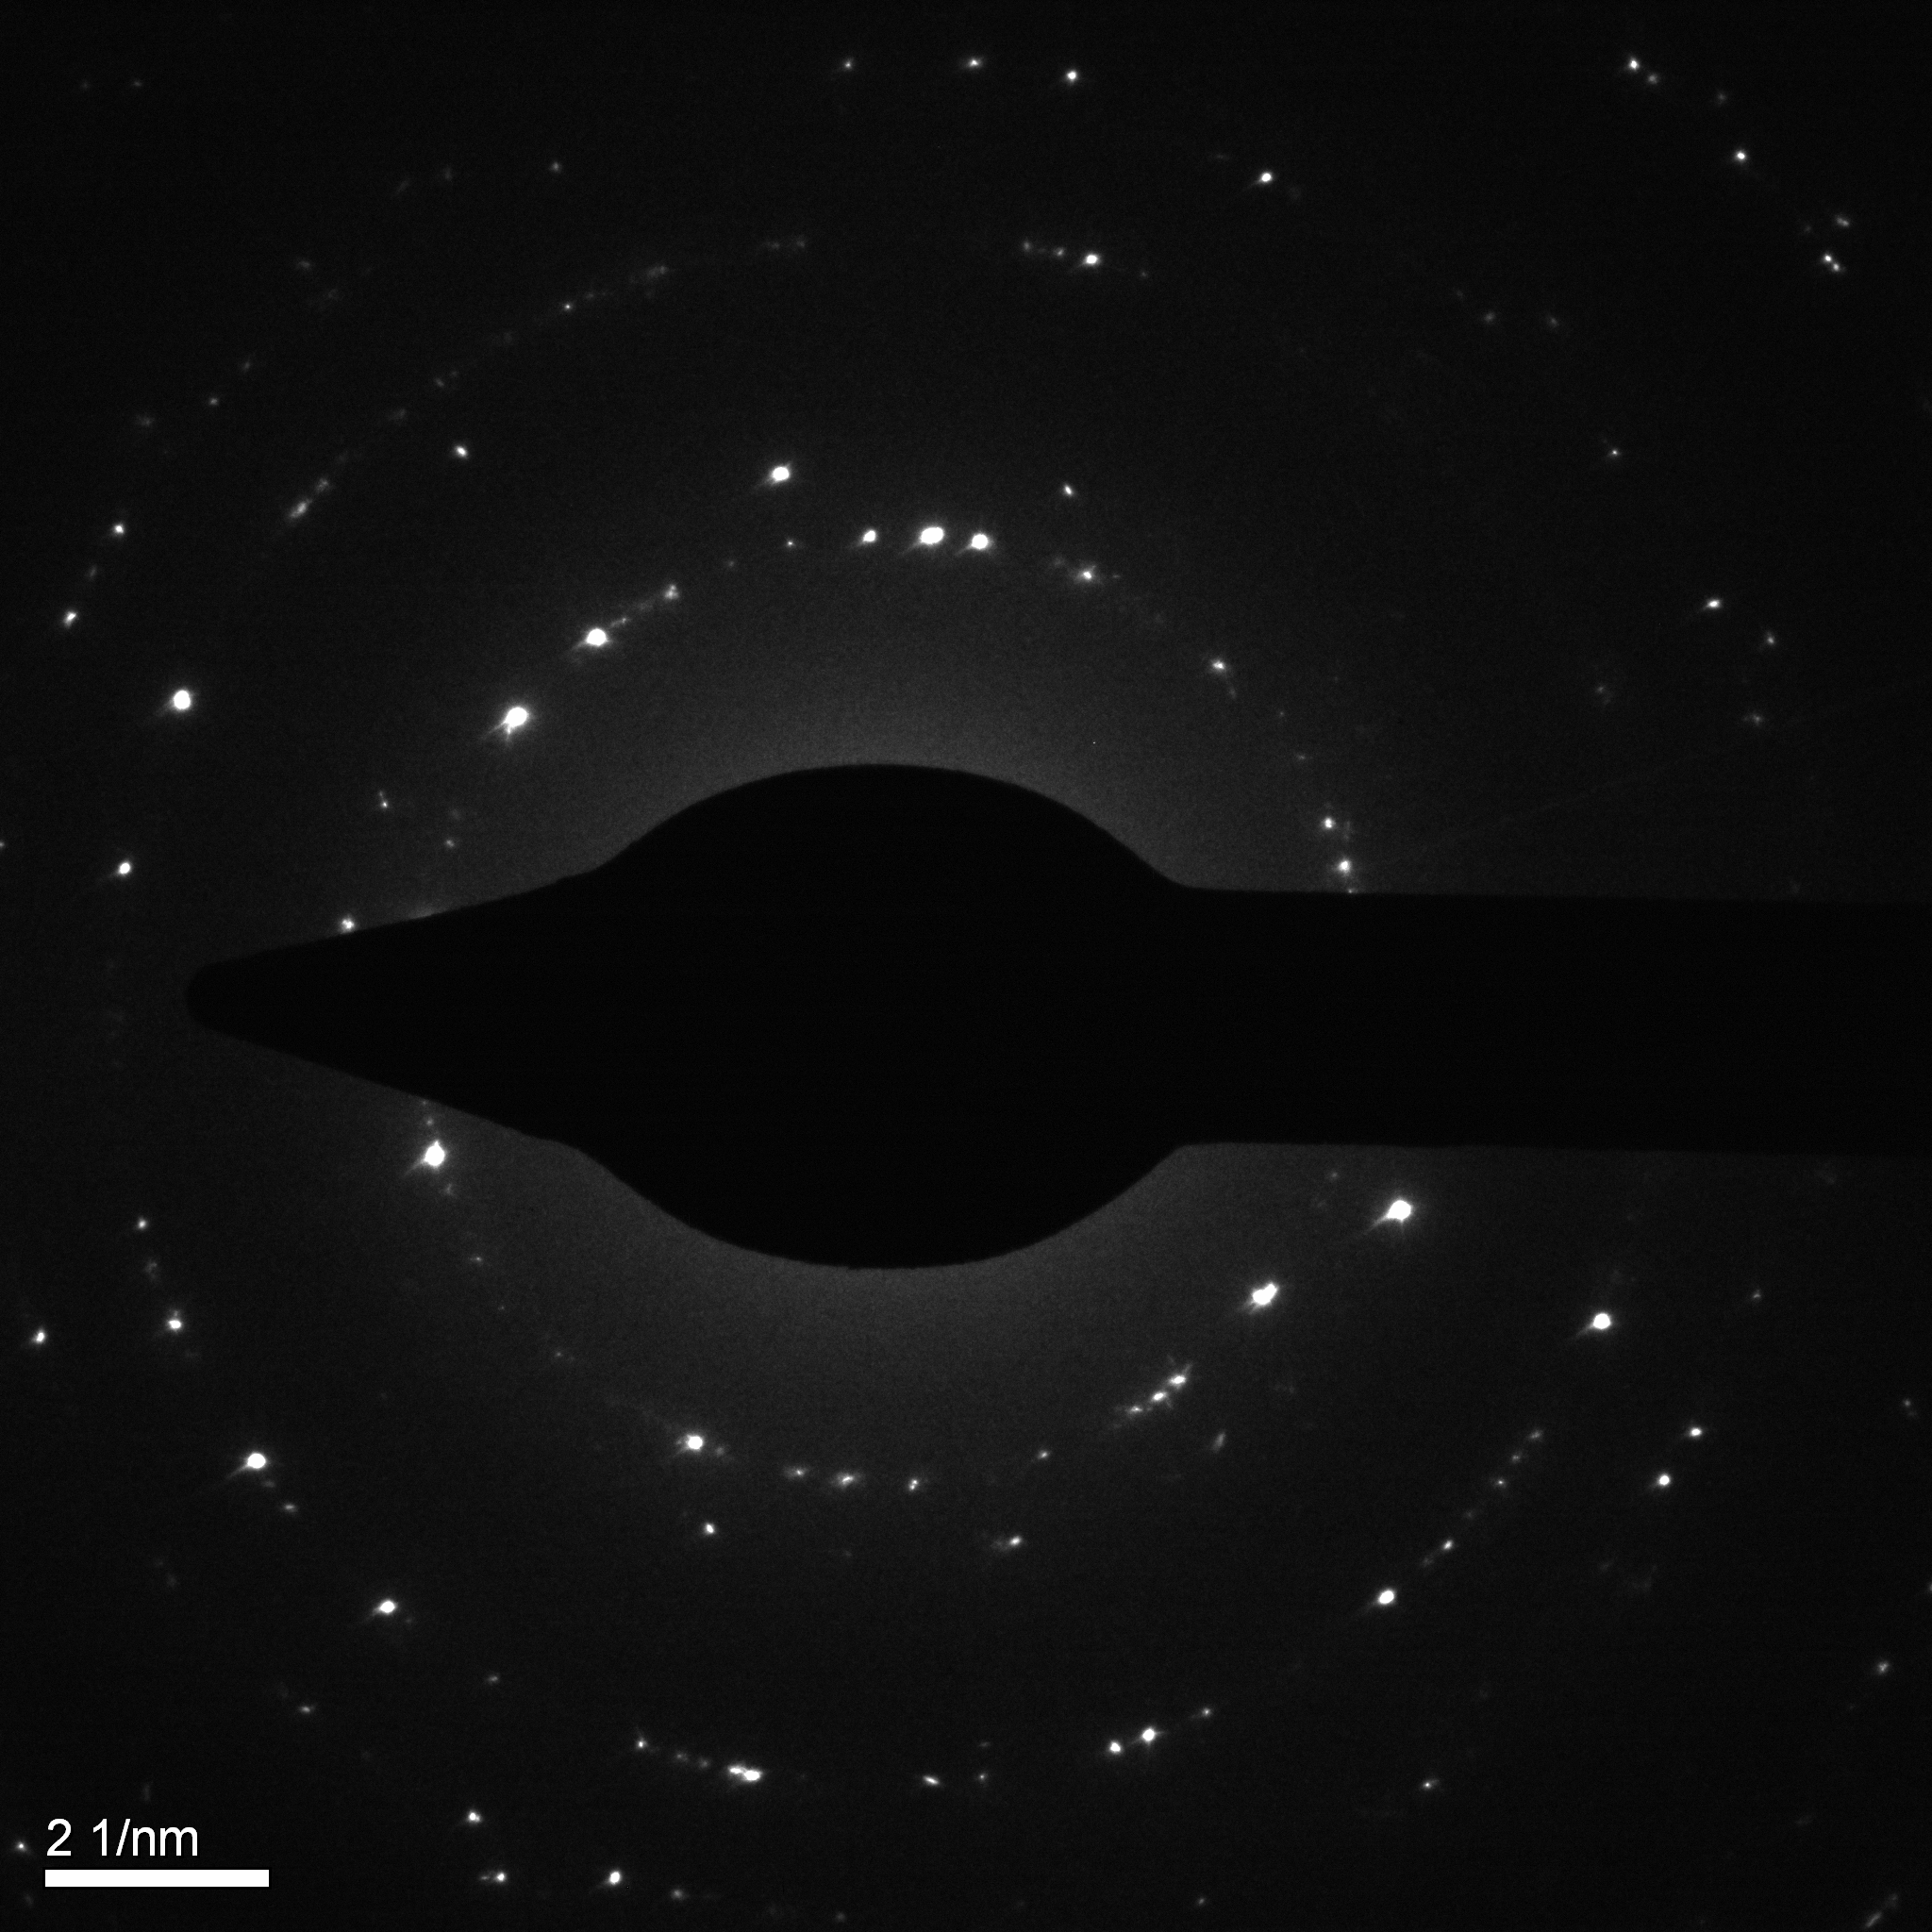
\includegraphics[width=\textwidth]{data/Image1 Al_Diff_SAED2.png}
    \caption{aluminum polycrystalline pattern using SAED setting 2}
    \label{fig:al2}
  \end{subfigure}%
  ~
  \begin{subfigure}[b]{0.45\textwidth}
    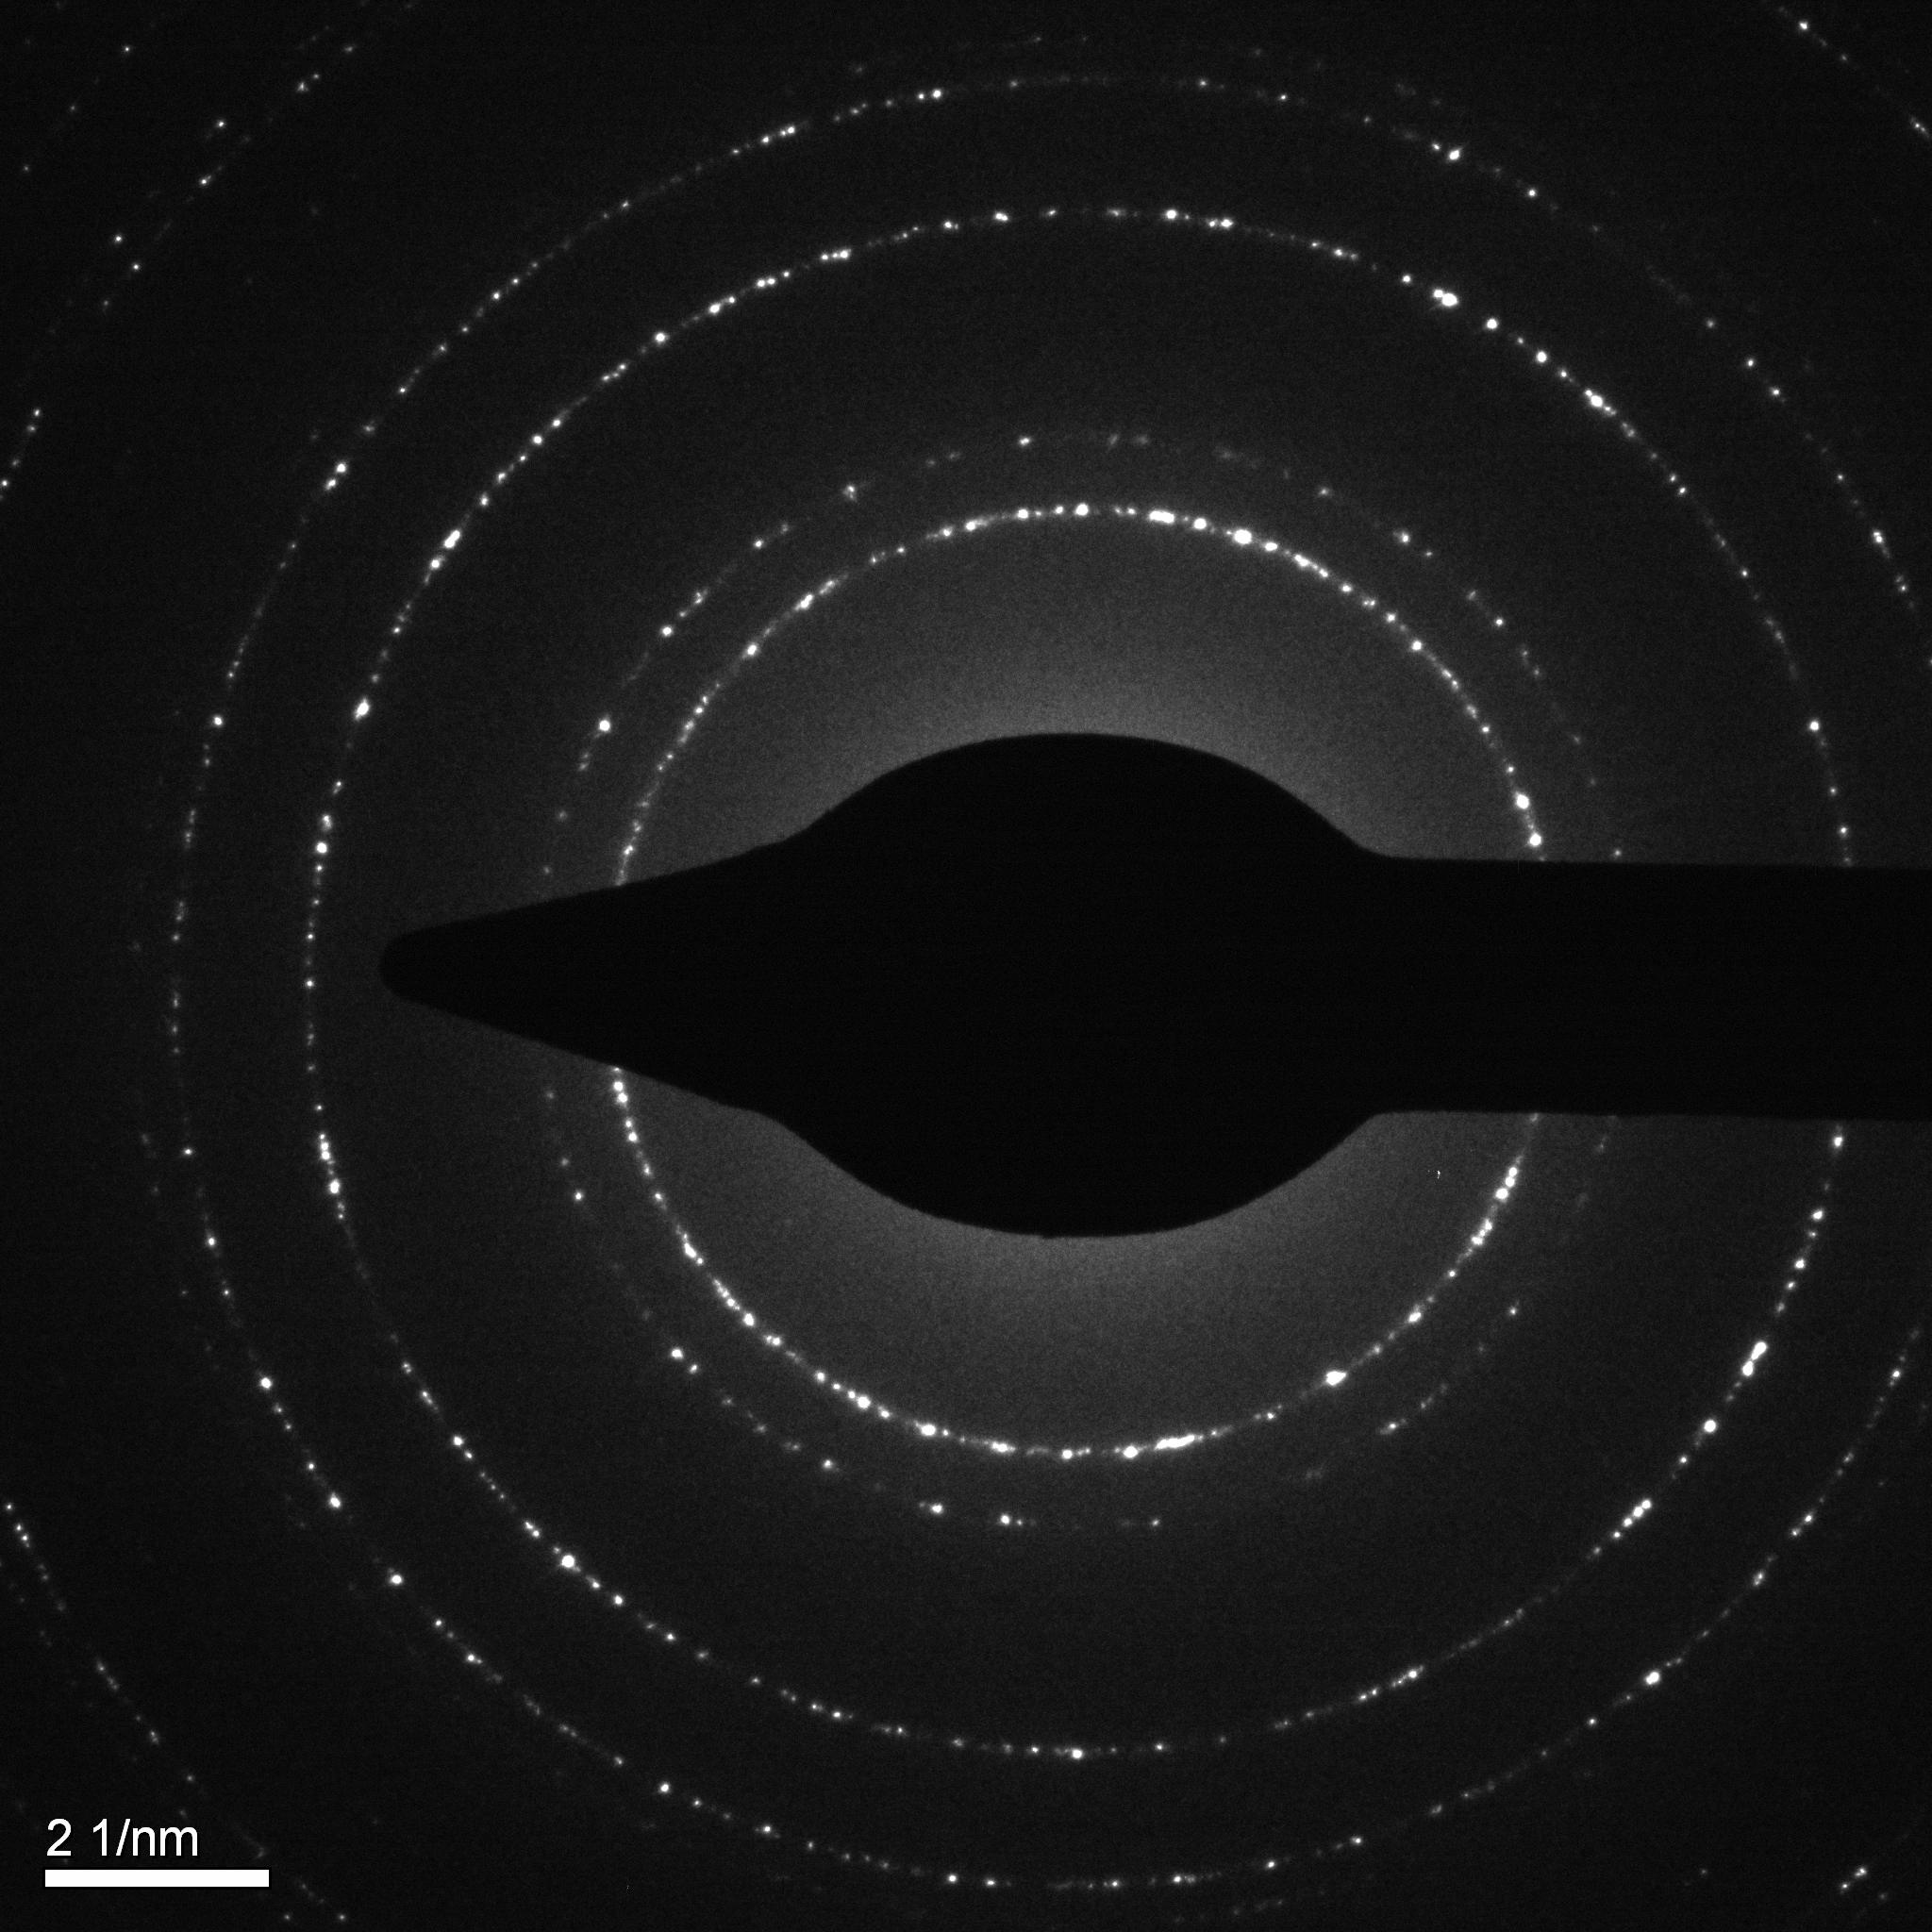
\includegraphics[width=\textwidth]{data/Image2Al_Diff_SAED3.png}
    \caption{aluminum polycrystalline pattern using SAED setting 3, }
    \label{fig:al3}
  \end{subfigure}
  \caption{Aluminum Polycrystalline Diffraction Patterns}
  \label{fig:aluminum}
\end{figure}

\begin{wrapfigure}{r}{0.5\textwidth}
  
\includegraphics[width=0.5\textwidth]{data/1024px-BraggPlaneDiffraction.svg.png}
  \caption{Illustrating the Bragg Condition\cite{wikibragg}.}
  \label{fig:d_space}
\end{wrapfigure}

The two different patterns are generated by changing the the \ac{saed} setting on the \ac{tem}.  By selecting different locations on the sample using this aperture described in \ref{sec:diffraction_pattern_formation}, we are able to see the different diffraction patterns from different structures on our sample.

By using a higher \ac{saed} setting, we can also decrees the brightness of the the bright spots seen in Figure~\ref{fig:al2}.  This can enhance the contrast of the dimmer points and allow us to take an image that contains more discernible detail.  Figure~\ref{fig:al3} appears brighter, but this is actually a result of imaging a darker, more contrast rich image with the reduction of the distinct bright points seen in Figure~\ref{fig:al2}.

\subsubsection{D Spacing} % (fold)
\label{ssub:d_spacing}

We can measure the $D$ spacing (the spacing between the planes of the atomic lattice structure) of our Aluminum polycrystalline sample due to the fact we are able to take a scaled image of our diffraction pattern.

We can do this by simply measuring the radius of the rings formed in our diffraction pattern.  The units of our image our in $\frac{1}{nm}$ so simply inverting this value will give us our actual spacing.

For image processing we use the ImageJ\cite{imagejs} software to scale our image, scale it correctly and then measure the area of the rings.  This can be seen in Table~\ref{tbl:rings}.  We see that the d-spacing is on the order of one or two angstroms, which matches what we would expect for the 1 1 1 planes of aluminum\cite{aluminum}.

\begin{table}[hct]
  \centering
  \begin{tabular}{c|c|c}
    \hline
    \hline
    Area ($1/nm^2$) & Radius ($1/nm$) & D Spacing ($nm$) \\
    \hline
    55.450 & 4.201 & 0.2380 \\
    74.963 & 4.884 & 0.2047 \\
    149.770 & 6.904   & 0.1448 \\
    \hline
    \hline
  \end{tabular}
  \caption{Measurements of Aluminum Polycrystalline Diffraction Pattern Seen in Figure~\ref{fig:al3} starting with the inner most ring.}
  \label{tbl:rings}
\end{table}

% subsubsection d_spacing (end)

% subsection ac (end)

\subsection{Single-Crystalline Silicon Diffraction Pattern} % (fold)
\label{sub:single_crystaline}

Looking at the single crystalline silicon sample we see a diffraction pattern with distinct points, rather than rings.  Using a reference image\cite{viz} of what the different diffraction patterns from the different crystal lattice planes looks like, we can identify the orientation of our two images.  

\begin{figure}[htbp]
  \centering
  \begin{subfigure}[b]{0.45\textwidth}
    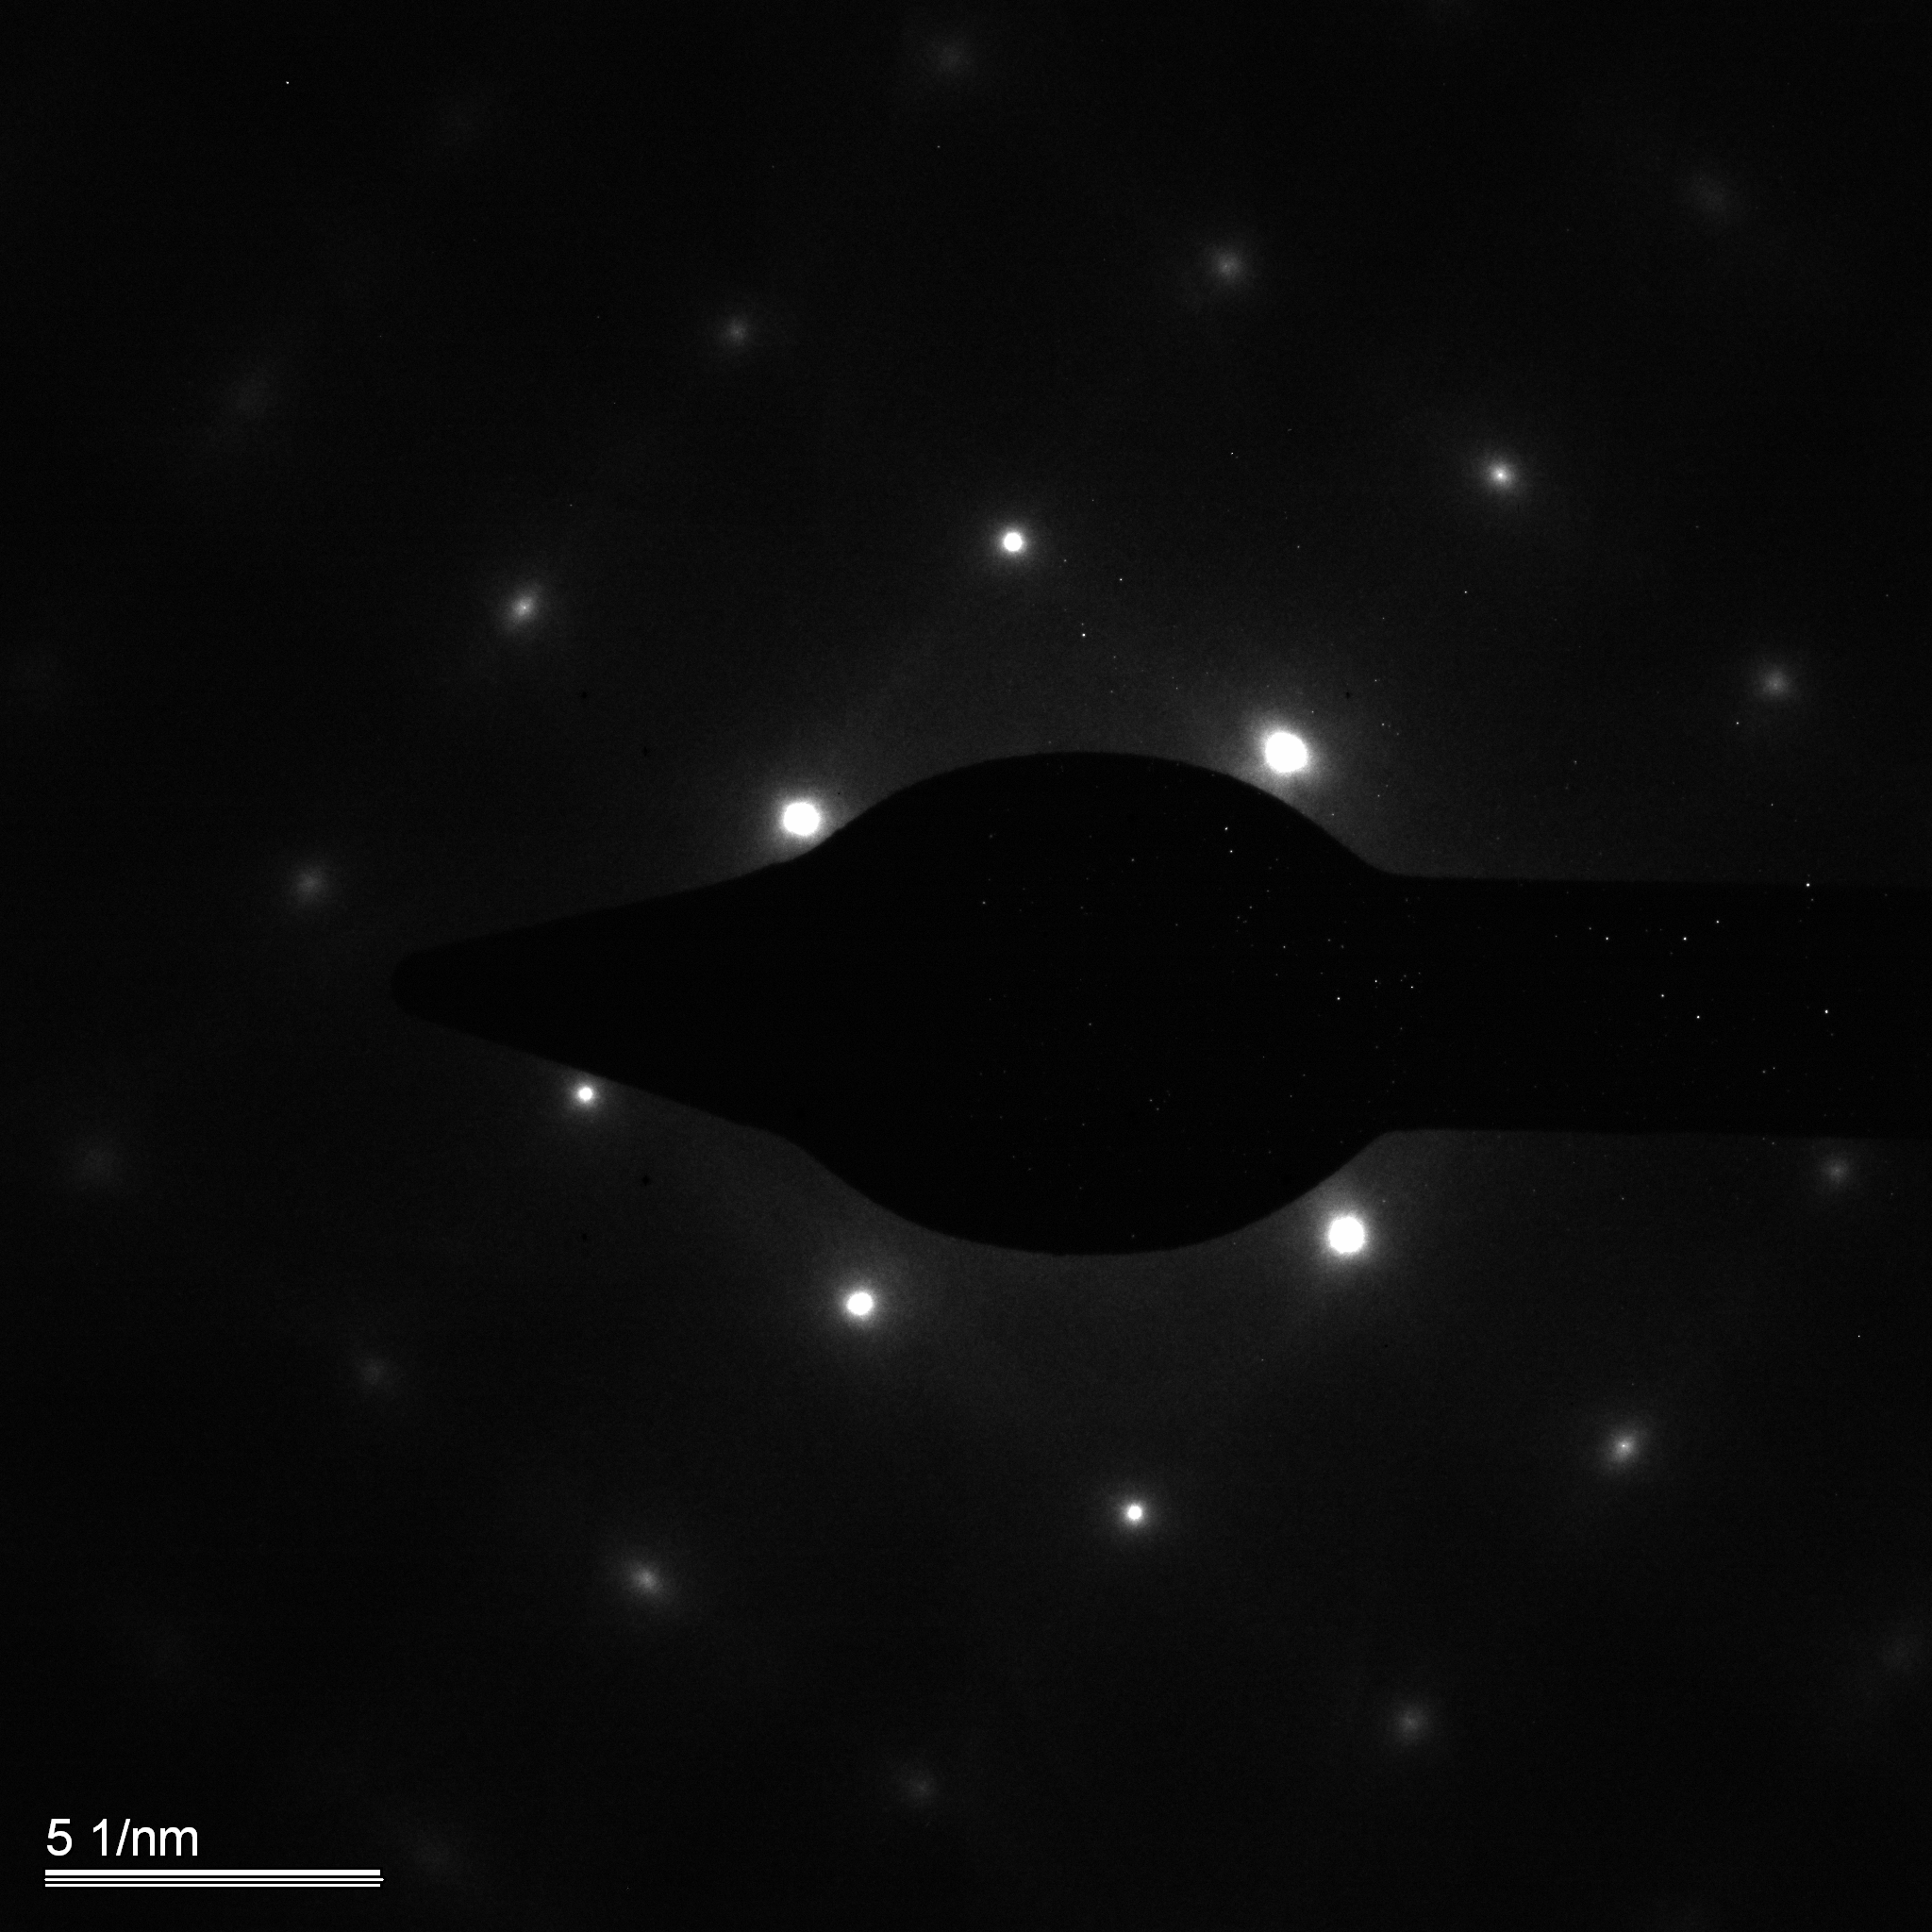
\includegraphics[width=\textwidth]{data/Image3 Si_Diff_Zone1.png}
    \caption{Single-crystalline Silicon Pattern 1}
    \label{fig:si1}
  \end{subfigure}%
  ~
  \begin{subfigure}[b]{0.45\textwidth}
    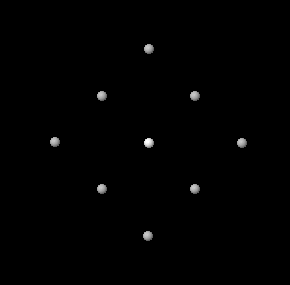
\includegraphics[width=\textwidth]{data/100.png}
    \caption{1 0 0 Reference Pattern}
    \label{fig:100}
  \end{subfigure}%
  \caption{Single-crystalline Silicon Pattern at one zone axis}
  \label{fig:zone1}
\end{figure}

Figure~\ref{fig:zone1} looks most similar to the $1 0 0$ reference images found in our reference simulation\cite{viz}.  We can see the edges of the square like pattern made and the right most corner and center are covered by the beam blocker.    There are a few other points that are clearly visible, but from the reference planes explored, this seemed to line up the best.

\begin{figure}[htbp]
  \centering
  \begin{subfigure}[b]{0.45\textwidth}
    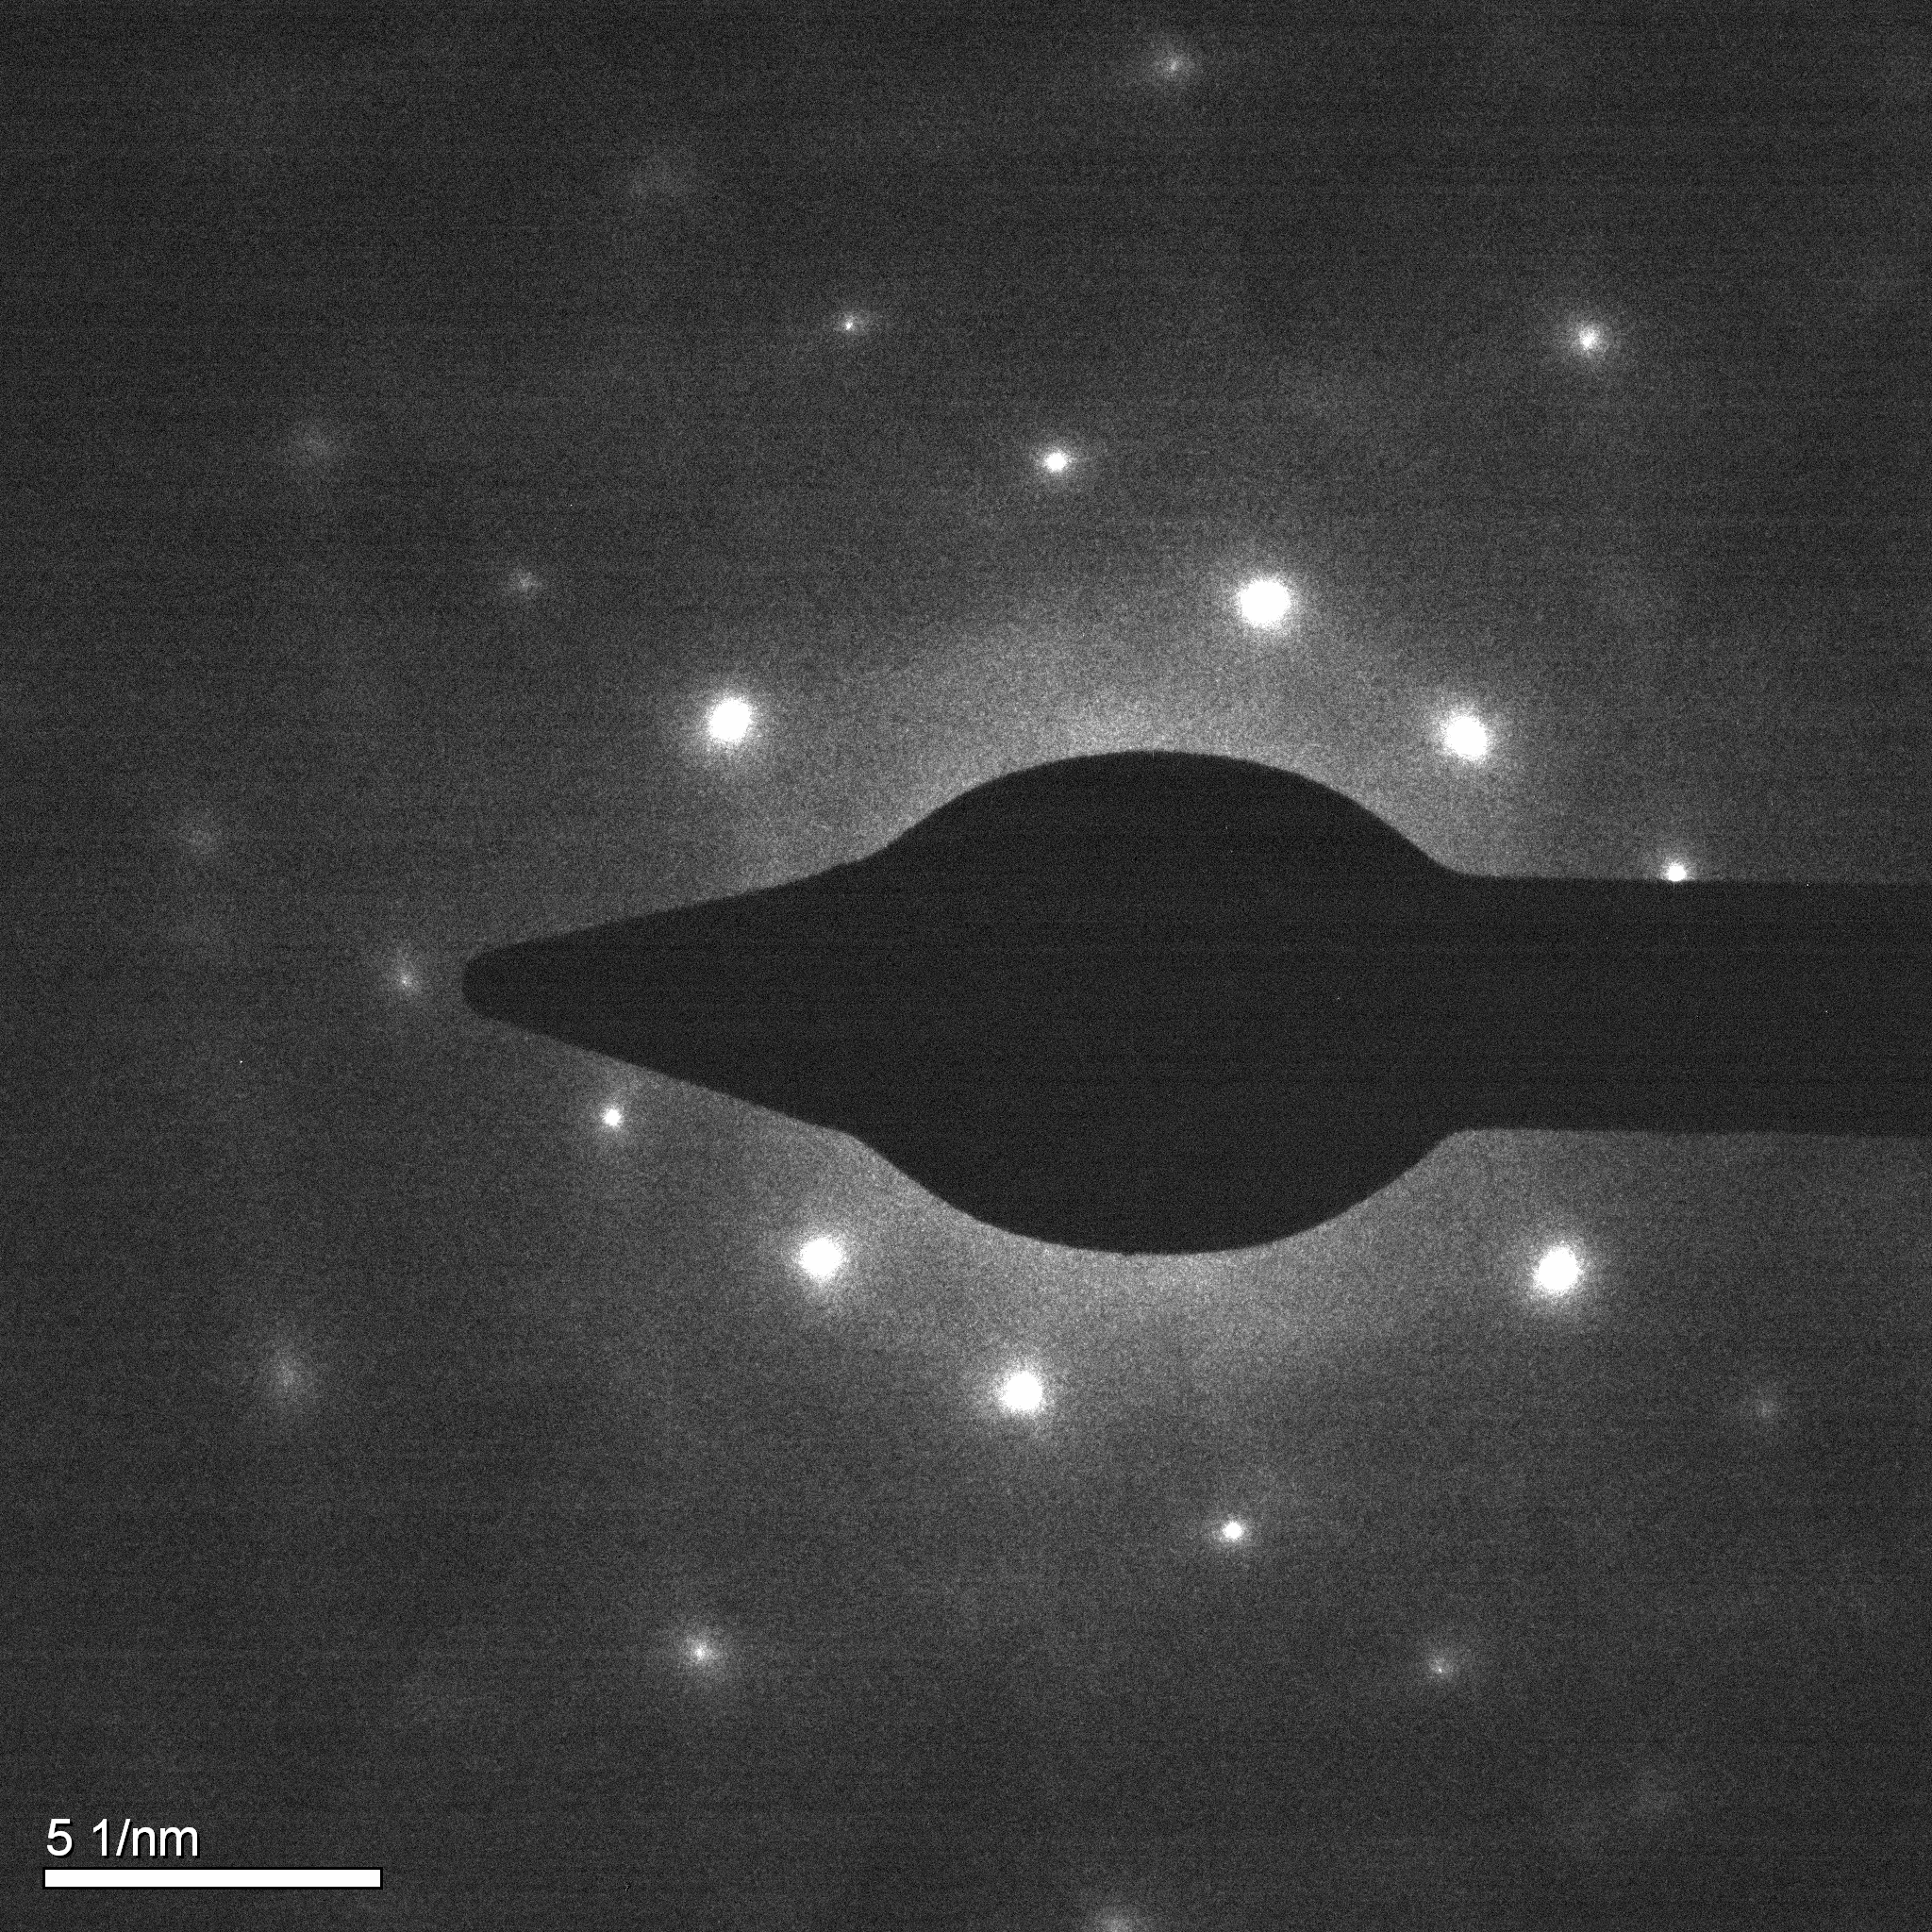
\includegraphics[width=\textwidth]{data/Image4 Si_Diff_Zone2.png}
    \caption{Single-crystalline Silicon Pattern 2}
    \label{fig:si2}
  \end{subfigure}
  ~
  \begin{subfigure}[b]{0.45\textwidth}
    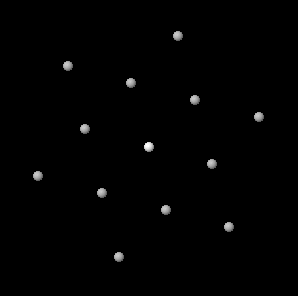
\includegraphics[width=\textwidth]{data/111.png}
    \caption{1 1 1 Reference Pattern}
    \label{fig:111}
  \end{subfigure}%
  \caption{single-crystalline silicon pattern at another zone axis}
  \label{fig:zone2}
\end{figure}

The second image is trickier but it looked closes to the $1 1 1 $ orientation.  It has a similar diamond shape to the $1 1 1$ pattern, but there appears to be additional diffraction points on top of it, or we have not found a sufficient orientation match.  Still,  if you exclude two of the bright points below the upper right and lower left star points, it is a pretty close match.

% subsection single_crystaline_ac (end)

\begin{figure}[htbp]
  \centering
  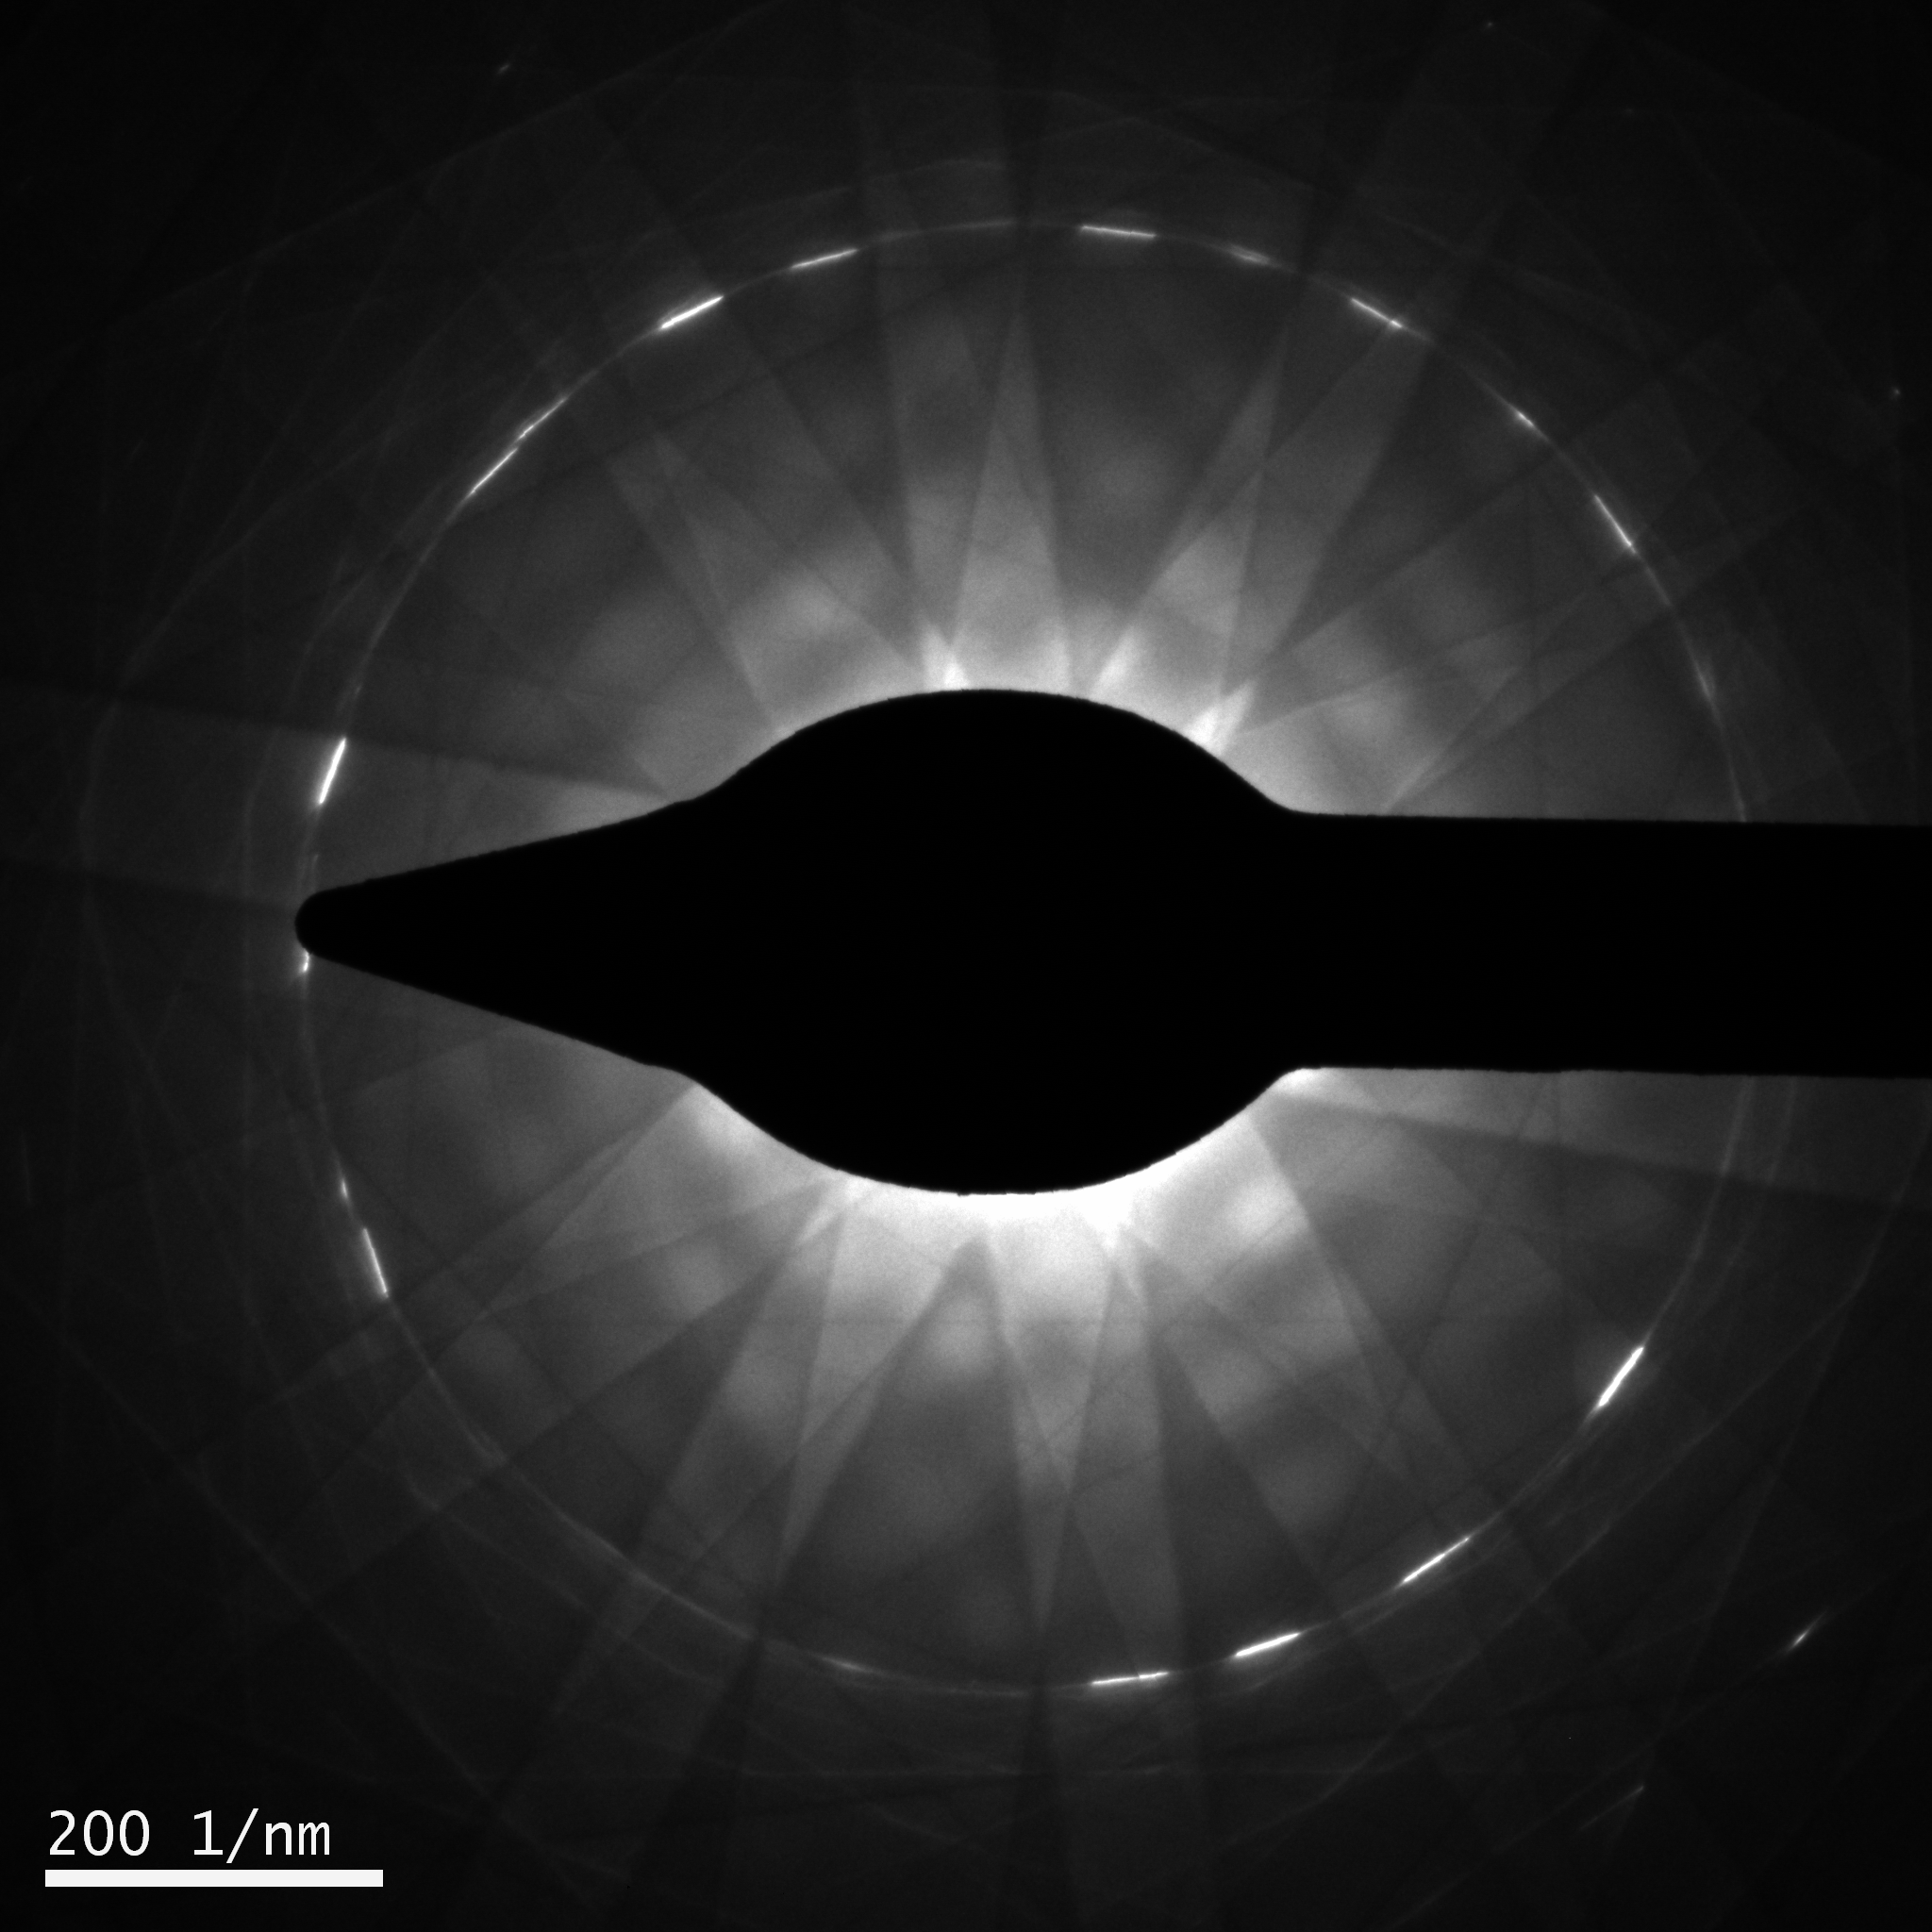
\includegraphics[width=0.6\textwidth]{data/Image6 Si_Kikuchi.png}
  \caption{Silicon Kikuchi pattern}
  \label{fig:kikuchi}
\end{figure}

\section{Lattice Spacing of Gold Foil Sample} % (fold)
\label{sec:lattice_spacing_of_gold_foil_sample}

By using our objective aperture, we are able to take high resolution images of the lattice structure of a gold foil sample.  This image is seen in Figure~\ref{fig:hr_au}.

\begin{figure}[htbp]
  \centering
  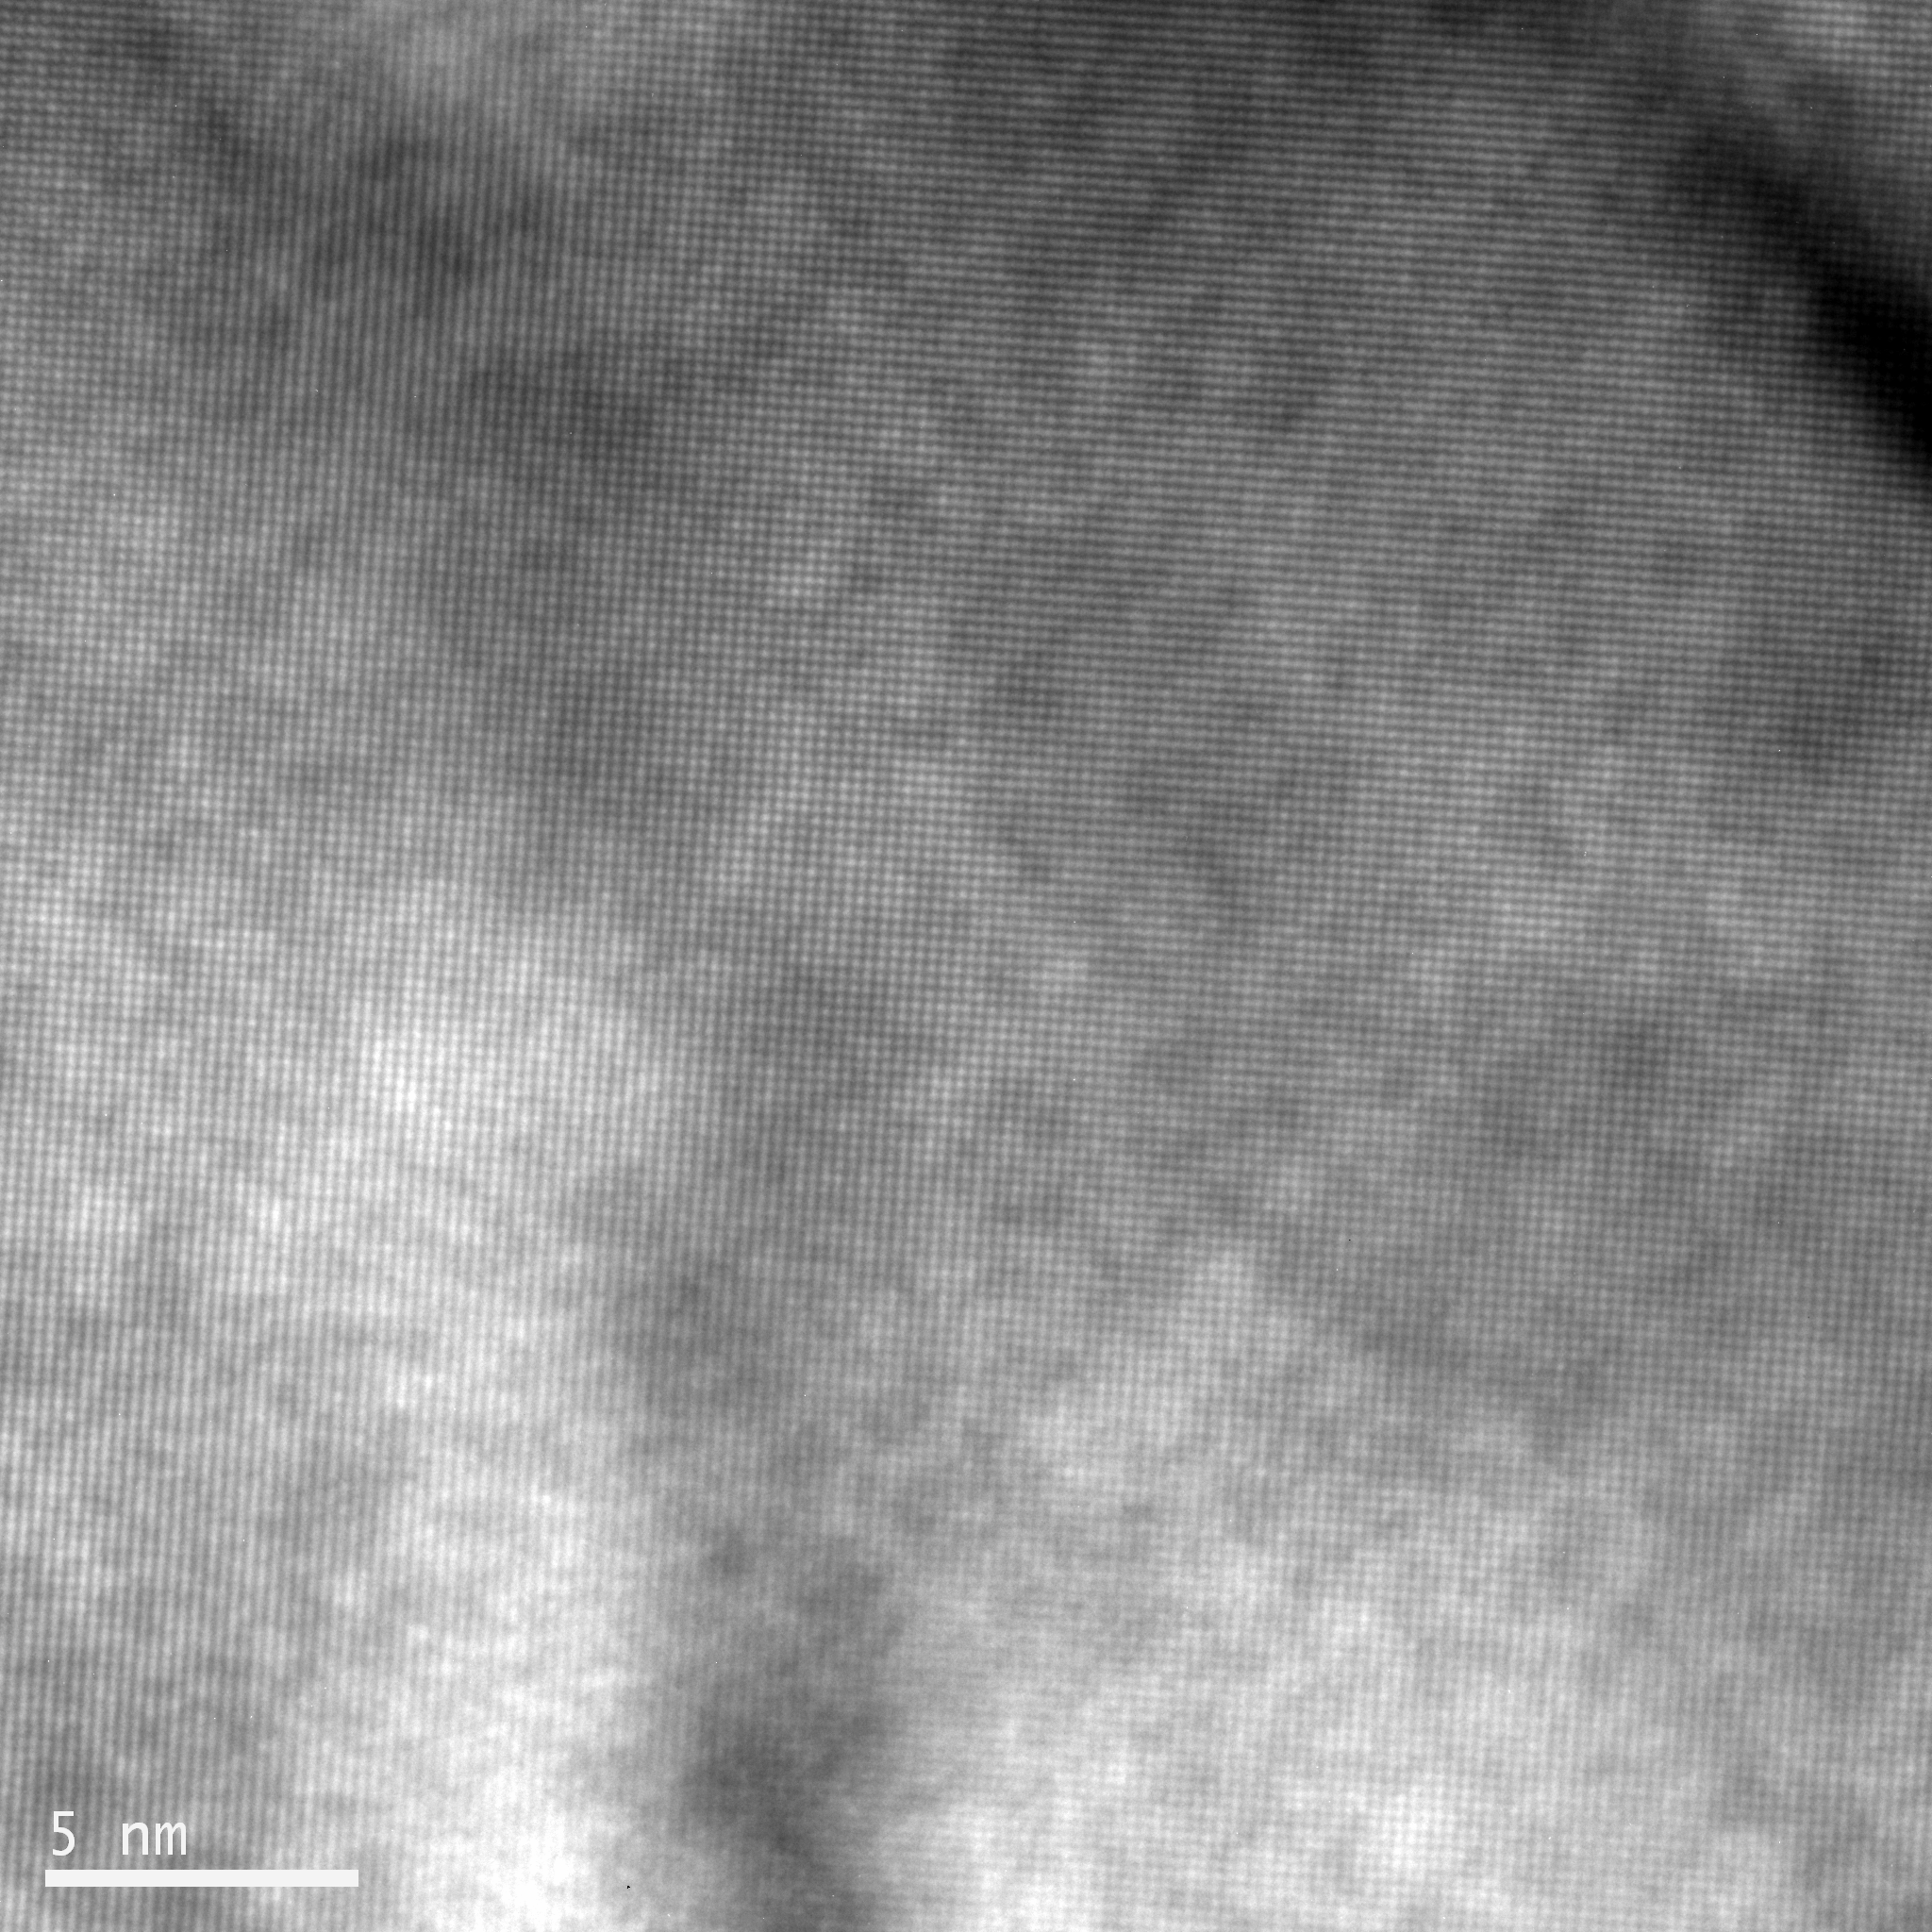
\includegraphics[width=0.6\textwidth]{data/Image5 Au_HRTEM.png}
  \caption{Gold ffoil \ac{hr} image}
  \label{fig:hr_au}
\end{figure}

Following a similar procedure as above, we scale our image using ImageJ, then take a measurement using our scaled image processing tools. This process is assisted by measuring the intensity of pixes to line up our ruler correctly as seen in Figure~\ref{fig:profile}

\begin{wrapfigure}{r}{0.45\textwidth}
  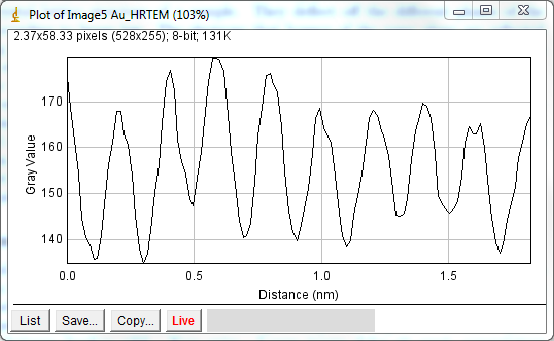
\includegraphics[width=0.45\textwidth]{data/Image5 Au_HRTEM profile.png}
  \caption{ImageJ profiling tools}
  \label{fig:profile}
\end{wrapfigure}

Measuring 10 fringe points we found a length of $1.827 nm$ which give us a D-spacing of $0.1827 nm$. This is fairly close to the $2 0 0$ orientation\cite{aluminum}.

% section lattice_spacing_of_gold_foil_sample (end)

\section{Conclusion} % Major section

We were able to measure the d-spacing of the polycrystalline aluminum sample using the diffraction pattern as well as find the orientation of our silicon sample by matching it to reference patterns at known orientations.  Finally we directly measured the d-spacing of gold foil by using a high resolution TEM image.

\bibliography{references-3} 
\bibliographystyle{plain} \nocite{*}

\end{document}